\section{Ejercicios de aplicacion en ingeniería}
\begin{enumerate}
    \item Un sensor mide la velocidad de un vehículo cada 5 segundos. Aproximar la distancia recorrida con sumas de Riemann.
\end{enumerate}

\[
x(t) = x_0 + v_0 t + \frac{1}{2} a t^2
\]

\[
\frac{d x}{dt} = V(t) = v_0 + a t
\]

\[
\frac{d^2 x}{dt^2} = \frac{dV}{dt} = a
\]

\[
t_0 \quad t_1 \quad t_2 \quad t_3 \quad \dots \quad t_f
\]

\[
V(t_0) \quad V(t_1) \quad V(t_2) \quad V(t_3) \quad \dots \quad V(t_f)
\]

\[
K = 5 \quad V(t_i) = v_0 + a t_i
\]

\[
t_i = a + k i = 5i
\]

\[
\int_{t_0}^{t_f} V(t) \, dt = x(t) = \lim_{n \to \infty} k \sum_{i=1}^{n} V(t_i)
\]

\[
= \lim_{n \to \infty} 5 \sum_{i=1}^{n} \left( v_0 + a t_i \right)
\]

\[
= \lim_{n \to \infty} \left[ 5 v_0 \sum_{i=1}^{n} 1 + 5 a \sum_{i=1}^{n} 5 i \right]
\]

\[
= \lim_{n \to \infty} \left[ 5 n v_0 + 25 a \sum_{i=1}^{n} i \right]
\]

\[
= \lim_{n \to \infty} \left[ 5 n v_0 + 25 a \cdot \frac{n(n+1)}{2} \right]
\]

\[
= \infty + \infty = \infty
\]

\textbf{Conclusión}: La distancia recorrida por el carro tiende al infinito, pues si
el sensor toma la velocidad cada 5 segundos durante un tiempo indefinido,
entonces las distancias se suman y cada vez se hacen más grandes.

\begin{enumerate}
    \setcounter{enumi}{1}
    \item En un sistema de enfriamiento, la temperatura varía con el tiempo según $T(t) = e^{-t}$. Calcule la cantidad total de calor disipado en 10 segundos usando el método del trapecio.
\end{enumerate}

\[
\int_{0}^{10} e^{-t} \, dt
\]

\[
f(t) = e^{-t}
\]

\textbf{Método del trapecio:}

\[
\frac{k}{2} \sum_{i=1}^{n} \left( f(x_{i-1}) + f(x_i) \right) \quad \text{si } n \text{ es par}
\]

\[
\frac{k}{2} \left[ f(x_0) + 2f(x_1) + 2f(x_2) + 2f(x_i) + f(x_n) \right]
\]

\[
\frac{k}{2} f(x_0) + k \sum_{i=1}^{n-1} f(x_i) + \frac{k}{2} f(x_n)
\]

\begin{figure}[H]
\centering
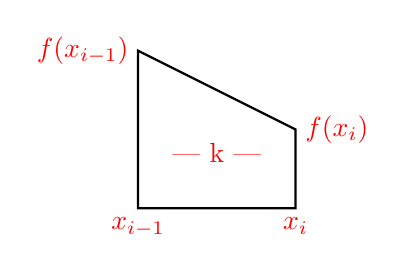
\begin{tikzpicture}
    % Definir los puntos
    \coordinate (A) at (0,2);
    \coordinate (B) at (2,1);
    \coordinate (C) at (2,0);
    \coordinate (D) at (0,0);
    
    % Dibujar el trapecio
    \draw [thick] (A) -- (B) -- (C) -- (D) -- cycle;
    
    % Etiquetas de funciones
    \node[left] at (A) {\textcolor{red}{$f(x_{i-1})$}};
    \node[right] at (B) {\textcolor{red}{$f(x_i)$}};
    \node[below] at (D) {\textcolor{red}{$x_{i-1}$}};
    \node[below] at (C) {\textcolor{red}{$x_i$}};

    % Línea y etiqueta de k dentro del trapecio
    \node[red] at (1,0.7) {\textemdash\ k\ \textemdash};  

\end{tikzpicture}
\caption{Área del trapecio}
\end{figure}

\[
A = \frac{f(x_{i-1}) + f(x_i)}{2} k
\]

\textbf{Solución:}
\[
k = \frac{b-a}{n}
\]

\text{Cuando } n = 20

\[
k = \frac{10}{20} = \frac{1}{2}
\]

\[
t_i = a + k i
\]

\[
t_i = \frac{1}{2} i
\]

\[
f(t_i) = f(x_i) = e^{-\left(\frac{1}{2} i\right)}
\]

\text{Área con trapecios } = A

\[
A = \frac{k}{2} f(x_0) + k \sum_{i=1}^{n-1} f(x_i) + \frac{k}{2} f(x_n)
\]

\[
A = \frac{k}{2} e^{-\left(\frac{1}{2} \cdot 0\right)} + k \sum_{i=1}^{19} e^{-\left(\frac{1}{2} i\right)} + \frac{k}{2} e^{-\left(\frac{1}{2} \cdot 20\right)}
\]

\textbf{Propiedad:} $\quad x^{b \cdot c} = (x^b)^c$

\[
A = \frac{k}{2} \cdot 1 + k \sum_{i=1}^{19} \left( e^{-\frac{1}{2}i} \right) + \frac{k}{2} e^{-10}
\]

\textbf{Propiedad:} 

\[
\sum_{i=0}^{n} x^i = \frac{1 - x^{n+1}}{1 - x}
\]

Si $i = j \Rightarrow$ y $j > 1$

\[
\sum_{i=j}^{n} x^i = \sum_{i=0}^{n} x^i - \sum_{i=0}^{j-1} x^i
\]

\[
\sum_{i=j}^{n} x^i = \frac{1 - x^{n+1}}{1 - x} - \frac{1 - x^j}{1 - x}
\]

\text{Dado que } j-1+1 = j = i, \text{ entonces:}

\begin{equation}
\sum_{i=j}^{n} x^i = \frac{1 - x^{n+1}}{1 - x} - \frac{1 - x^i}{1 - x}
\label{eq:sumatoria}
\end{equation}

\[
\text{Si } \left( e^{\frac{1}{2}} \right) = x \quad \Rightarrow \quad \left( e^{-\frac{1}{2}} \right)^i = x^i
\]

\[
\sum_{i=1}^{19} \left( e^{-\frac{1}{2}} \right)^i = \frac{1 - \left(e^{-\frac{1}{2}}\right)^{20}}{1 - \left(e^{-\frac{1}{2}}\right)}
\]

\[
\sum_{i=1}^{19} \left( e^{-\frac{1}{2}} \right)^i = \frac{1 - \left(e^{-\frac{1}{2}}\right)^{20}}{1 - \left(e^{-\frac{1}{2}}\right)} - 1
\]

\[
A = \frac{k}{2} \cdot 1 + k \sum_{i=1}^{19} \left( e^{-\frac{1}{2} i} \right) + \frac{k}{2} e^{-10}
\]

\[
A = \frac{k}{2} + k \cdot \frac{1 - \left(e^{-\frac{1}{2}}\right)^{20}}{1 - e^{-\frac{1}{2}}} - 1 + \frac{k}{2} e^{-10}
\]

\[
A = k \left[ \frac{1}{2} + \left( \frac{1 - \left(e^{-\frac{1}{2}}\right)^{20}}{1 - e^{-\frac{1}{2}}} - 1 \right) + \frac{1}{2} e^{-10} \right]
\]

\[
A = \frac{1}{2} \left[ \frac{1}{2} + \left( \frac{1 - \left(e^{-\frac{1}{2}}\right)^{20}}{1 - e^{-\frac{1}{2}}} - 1 \right) + \frac{1}{2} e^{-10} \right]
\]

\[
A = 1.020700699 u^2 \quad \text{para } n = 20
\]
